\PassOptionsToPackage{hyphens}{url}
\documentclass[11pt,a4paper]{article}

\usepackage[utf8]{inputenc}
\usepackage[spanish,es-nodecimaldot,es-tabla]{babel}
\usepackage[T1]{fontenc}
\usepackage{lmodern}
\usepackage[margin=2.35cm]{geometry}
\usepackage{amsmath}
\usepackage{amssymb}
\usepackage{booktabs}
\usepackage{longtable}
\usepackage{tabularx}
\usepackage{array}
\usepackage{enumitem}
\usepackage{listings}
\usepackage{xcolor}
\usepackage{microtype}
\usepackage{parskip}
\usepackage{titlesec}
\usepackage{hyperref}
\usepackage{graphicx}
\usepackage{caption}
\usepackage{float}
\usepackage{tocloft}
\setlength{\cftsecnumwidth}{2.2em}
\setlength{\cftsubsecnumwidth}{2.8em}

\definecolor{azulWCD}{RGB}{17,67,112}
\definecolor{grisCodigo}{RGB}{247,247,247}
\definecolor{tituloColor}{RGB}{0,55,110}
\definecolor{reglaColor}{RGB}{0,90,160}

\hypersetup{colorlinks=true, linkcolor=azulWCD, urlcolor=azulWCD, citecolor=azulWCD,
  pdftitle={Respuesta electromagnética del WCD a la captura de neutrones: carga y eficiencia}, pdfauthor={Jaime A. Betancourt}}

\lstdefinestyle{shstyle}{backgroundcolor=\color{grisCodigo}, basicstyle=\ttfamily\footnotesize, breaklines=true,
  frame=single, rulecolor=\color{gray!40}, columns=fullflexible, keepspaces=true}
\lstset{style=shstyle}

\titleformat{\section}{\normalfont\Large\bfseries\color{azulWCD}}{\thesection.}{0.6em}{}
\titleformat{\subsection}{\normalfont\large\bfseries}{\thesubsection.}{0.5em}{}
\setlist{itemsep=0.25em,topsep=0.4em}
\renewcommand{\arraystretch}{1.18}
\setlength{\emergencystretch}{2em}
\captionsetup{font=small,labelfont=bf}
\renewcommand{\cftsecfont}{\bfseries\color{azulWCD}}
\renewcommand{\cftsecpagefont}{\bfseries}

\graphicspath{{../../../analysis/campana-1_respuesta-electromagnetica_seccion-4.2/figuras-carga/}}
\newcommand{\tablas}{tablas-carga}
\usepackage{url}
\DeclareUrlCommand\archivo{\urlstyle{tt}}
\newcommand{\var}[1]{\texttt{#1}}

\begin{document}
\pagestyle{empty}

\begin{titlepage}
\begin{center}
\vspace*{0.5cm}
\textcolor{reglaColor}{\rule{\linewidth}{1.2pt}}

\vspace{1.3cm}
{\Large\scshape Universidad Industrial de Santander}\\[0.2cm]
{\large Escuela de Física --- Facultad de Ciencias}\\[0.2cm]
{\large Doctorado en Física}

\vspace{2.2cm}
{\Huge\bfseries\color{tituloColor} Respuesta electromagnética\\[0.3cm] del WCD a la captura\\[0.3cm] de neutrones}

\vspace{1.2cm}
{\Large Carga total y eficiencia de detección}

\vspace{1.4cm}
{\large\textbf{Informe técnico}}

\vspace{0.6cm}
\begin{minipage}{0.82\linewidth}
\centering
\textit{``Distribución de la carga por evento, eficiencia de detección y su relación con la captura del neutrón en agua pura y en agua con NaCl para neutrones de 1~meV a 1~keV (Campaña~1, dieciséis energías)''}
\end{minipage}

\vfill
{\large\textbf{Autor}}\\[0.15cm]
Jaime A. Betancourt\\[0.1cm]
Doctorado en Física, Universidad Industrial de Santander

\vspace{1.2cm}
\textcolor{reglaColor}{\rule{0.5\linewidth}{0.6pt}}

\vspace{1cm}
9 de octubre de 2026

\vspace{1cm}
\textcolor{reglaColor}{\rule{\linewidth}{1.2pt}}
\end{center}
\end{titlepage}

\pagestyle{plain}

\begin{abstract}
Este informe estudia el último eslabón de la respuesta del detector Cherenkov de agua (WCD) a la captura de neutrones de la Campaña~1: la carga total por evento (fotoelectrones, pe) y la eficiencia de detección. Se cubren dieciséis energías entre 1~meV y 1~keV y cuatro medios: agua pura y agua con 2.5, 5 y 10~\% de NaCl, con $10^5$ neutrones por corrida y \texttt{QGSP\_BERT\_HP} sin $S(\alpha,\beta)$. Los archivos de carga solo contienen los eventos con señal, así que su número de filas da directamente la eficiencia $\varepsilon(Q\geq1)$. Con las capturas de la parte neutrónica esa eficiencia se factoriza en $\varepsilon = \eta_\mathrm{Cap}\times P(\text{señal}\mid\text{captura})$.
Resultados principales:
(i)~la \emph{forma} de la distribución de carga y la carga media dependen solo del medio ($\langle Q\rangle\approx3.2$, 7.5, 9.1 y 10.5~pe) y no de la energía del neutrón: varían a lo sumo un 3~\% en seis décadas;
(ii)~la energía controla \emph{cuántos} eventos dan señal: $\varepsilon(Q\geq1)$ pasa de 8.0~\% a 1~meV a 18.0~\% a 1~eV en agua pura, y de 16.4~\% a 31.8~\% con 10~\% de NaCl, sobre todo porque cambia la fracción de captura;
(iii)~la probabilidad de señal por captura crece ligeramente con la energía (de 0.46 a 0.52 en agua pura), porque los neutrones más energéticos se capturan más hondo (de 2.9 a 5.1~cm bajo la superficie del agua) y escapan menos gammas;
(iv)~el NaCl multiplica la eficiencia por 1.25--2.0 con $Q\geq1$ y por 40--125 con $Q\geq20$~pe.
Como única anomalía, en el medio con 2.5~\% de NaCl la carga media es un 3~\% mayor por debajo de 10~meV ($5\sigma$). Este exceso no aparece en los demás medios y queda sin explicar.
\end{abstract}

\tableofcontents

% =====================================================================
\section{Objeto y alcance}

La Sección~4.2 de la tesis sigue la cadena que convierte cada captura en una señal,
\[
\mathrm{n}\;\longrightarrow\;\text{captura}\;\longrightarrow\;\gamma_\mathrm{Cap}\;\longrightarrow\;e^-,\,e^+\;\longrightarrow\;\text{radiación Cherenkov}\;\longrightarrow\;\mathrm{PMT}.
\]
Los eslabones anteriores están documentados en esta misma carpeta:
\begin{itemize}
  \item el transporte y la captura de los neutrones, en \emph{Respuesta del WCD a flujos monocromáticos de neutrones};
  \item los fotones de captura, en \emph{Respuesta electromagnética del WCD a la captura de neutrones: fotones gamma};
  \item los electrones, en \emph{\dots: electrones y positrones secundarios}.
\end{itemize}
Este informe trata la salida del detector: la carga que registra el PMT en cada evento y la fracción de neutrones que producen señal. Las Figs.~4.48, 4.50 y 4.51 de la tesis se regeneran en el notebook de la parte neutrónica; este informe las amplía. La producción y propagación de los fotones Cherenkov no se analiza aquí. Los objetivos son:
\begin{enumerate}
  \item caracterizar la distribución de carga en las 64 corridas y probar si depende de la energía del neutrón;
  \item medir la eficiencia de detección y separarla en captura y señal por captura;
  \item explicar la dependencia de la señal por captura con la profundidad a la que se captura el neutrón;
  \item cuantificar la ganancia de eficiencia del NaCl con distintos umbrales de carga.
\end{enumerate}

% =====================================================================
\section{Datos y método}

\subsection{Archivos de carga}

Cada corrida \archivo{Neutrones-termicos/<energía>/<medio>/} tiene un archivo \archivo{Carga\_Total\_*.txt} con un entero por fila: el número de fotoelectrones que producen en el PMT los fotones Cherenkov aceptados por su eficiencia cuántica. Dos observaciones:
\begin{itemize}
\item \textbf{Solo contienen eventos con señal.} Ningún archivo tiene $Q=0$. Como cada corrida lanza $N_0=10^5$ neutrones, el número de filas $N$ da la eficiencia $\varepsilon(Q\geq1)=N/N_0$, con error binomial $\sqrt{\varepsilon(1-\varepsilon)/N_0}\approx0.1$ puntos porcentuales.
\item \textbf{Procedencia.} \archivo{procesar\_corrida.py}, de la parte neutrónica, guarda el histograma de cada archivo en \archivo{resumen.json}. Una copia de trabajo de los 64 archivos, con otro esquema de nombres en nueve energías (\archivo{AP}, \archivo{A25NaCl}, \dots), resultó idéntica (suma MD5) a los originales.
\end{itemize}

\subsection{Captura y profundidad}

De la parte neutrónica se toman, por corrida, el número de capturas (\var{capturas} de \archivo{resumen.json}) y la posición de cada captura (\var{z\_cap} de \archivo{historias.tsv.gz}). Con ellas se calcula la profundidad bajo la superficie del agua ($z=1330$~mm) y las capturas fuera del agua ($z>1330$~mm). Estas últimas son solo el 0.1--1.6~\% del total, y la fracción es mayor a 1~meV. La profundidad media coincide con un cálculo independiente sobre \archivo{interaccion-completa-neutrones.txt}.

\subsection{Pruebas de dependencia con la energía}

Para cada medio se aplican dos pruebas:
\begin{enumerate}
\item un $\chi^2$ de las 16 cargas medias frente a su media ponderada (hipótesis: carga media constante);
\item una prueba $\chi^2$ de homogeneidad de los 16 histogramas completos. La tabla de contingencia es energía~$\times$~intervalo de carga, con 16 intervalos agrupados para que ninguna celda quede vacía.
\end{enumerate}
Además se compara la carga media del conjunto de energías bajas ($\leq10$~meV) con la de las altas ($\geq25$~meV).

% =====================================================================
\section{Distribuciones de carga}
\label{sec:histogramas}

\begin{figure}[H]
\centering
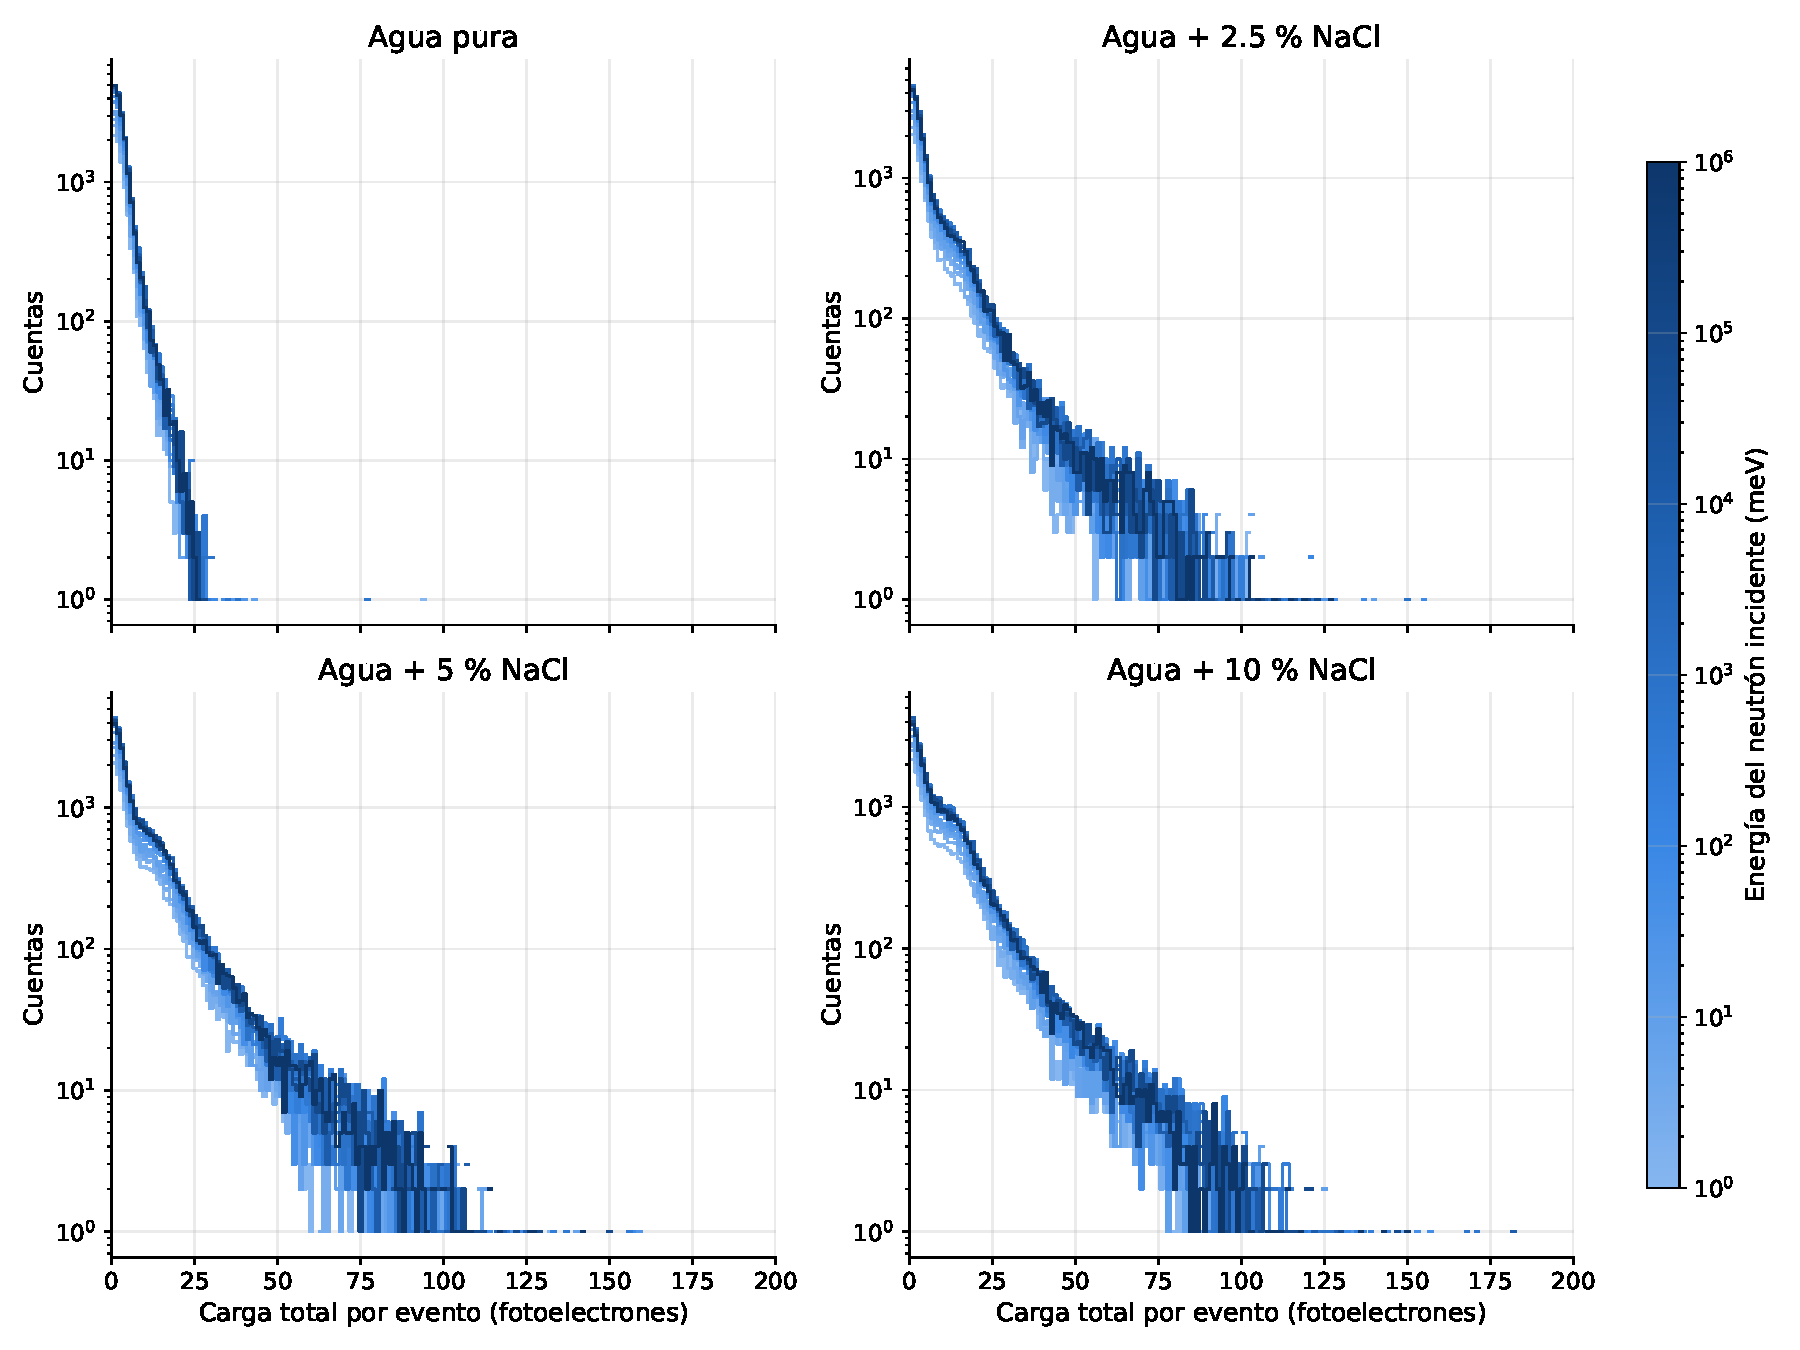
\includegraphics[width=\linewidth]{histograma_carga_matriz.pdf}
\caption{Histogramas de la carga total por evento (cuentas absolutas, bins de 1~pe, escala logarítmica). Un panel por medio y una curva por energía. El color va de azul claro (1~meV) a azul oscuro (1~keV) según la escala de la derecha.}
\label{fig:matriz}
\end{figure}

\begin{figure}[H]
\centering
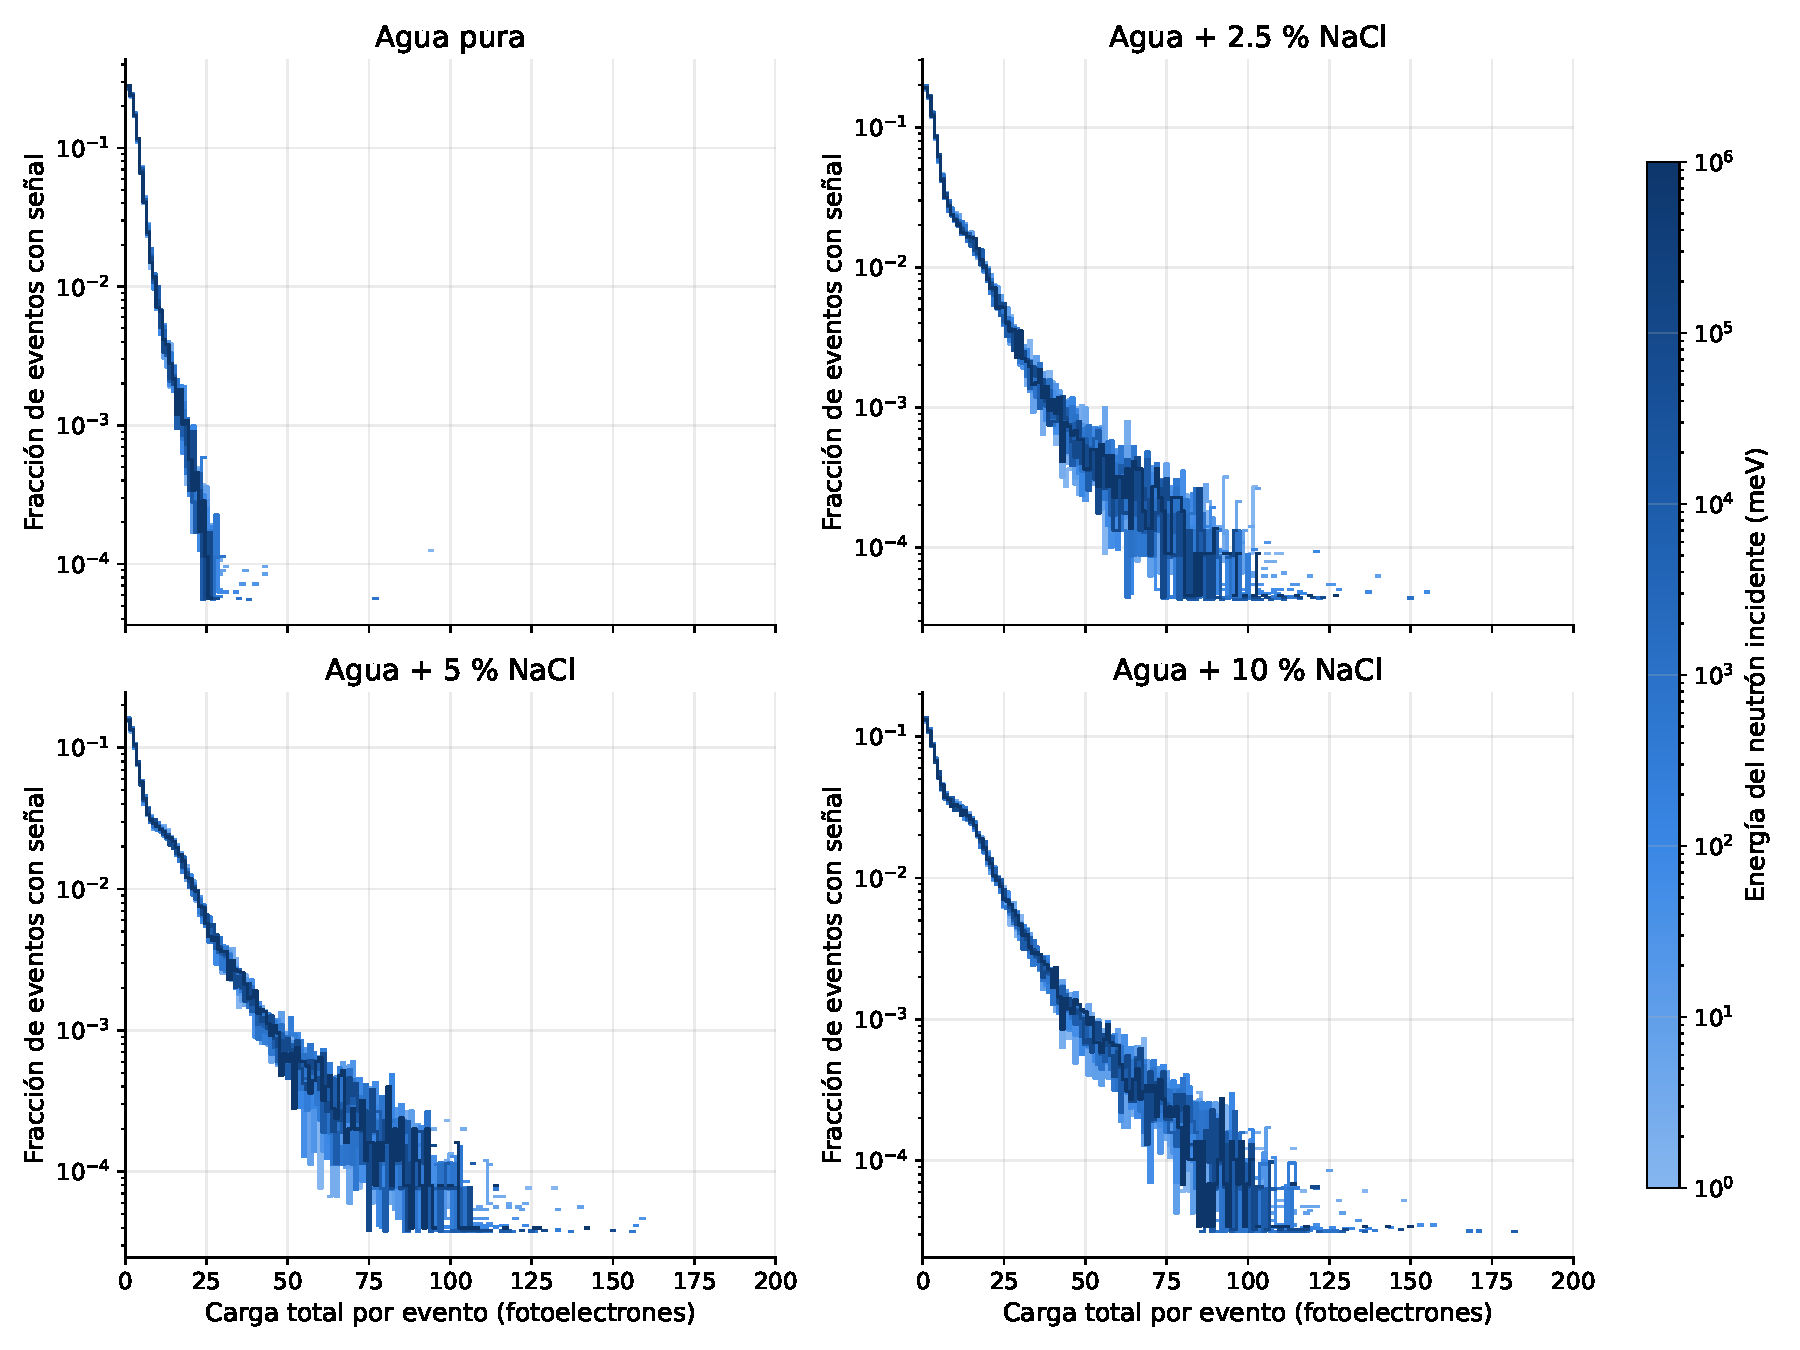
\includegraphics[width=\linewidth]{histograma_carga_matriz_normalizada.pdf}
\caption{Las mismas distribuciones normalizadas a la unidad (fracción de los eventos con señal). Al quitar la normalización, las 16 curvas de cada panel se superponen.}
\label{fig:matriz-norm}
\end{figure}

\begin{itemize}
\item \textbf{Forma.} Todas las distribuciones tienen su máximo en 1--2~pe y decaen de forma aproximadamente exponencial. En agua pura casi no hay eventos por encima de 25~pe: solo el 0.2--0.3~\% supera 20~pe. Los medios con NaCl muestran un \emph{hombro} entre $\sim$5 y $\sim$25~pe y una cola hasta 120--180~pe. Esa componente corresponde a la captura en $^{35}$Cl, cuya cascada de gammas suma $\approx8.6$~MeV, frente al único gamma de 2.2~MeV de la captura en hidrógeno. La fracción con $Q\geq20$~pe es $\approx8.6$, 11.7 y 14.6~\% para 2.5, 5 y 10~\% de NaCl.
\item \textbf{Efecto de la energía.} En la Figura~\ref{fig:matriz}, las curvas de baja energía (azul claro) quedan por debajo de las demás. Es un desplazamiento vertical, no un cambio de pendiente: al normalizar (Figura~\ref{fig:matriz-norm}) las curvas se superponen. La energía cambia el número de eventos con señal, no la carga que deja cada uno.
\end{itemize}

% =====================================================================
\section{Carga media e independencia de la energía}
\label{sec:carga}

\begin{figure}[H]
\centering
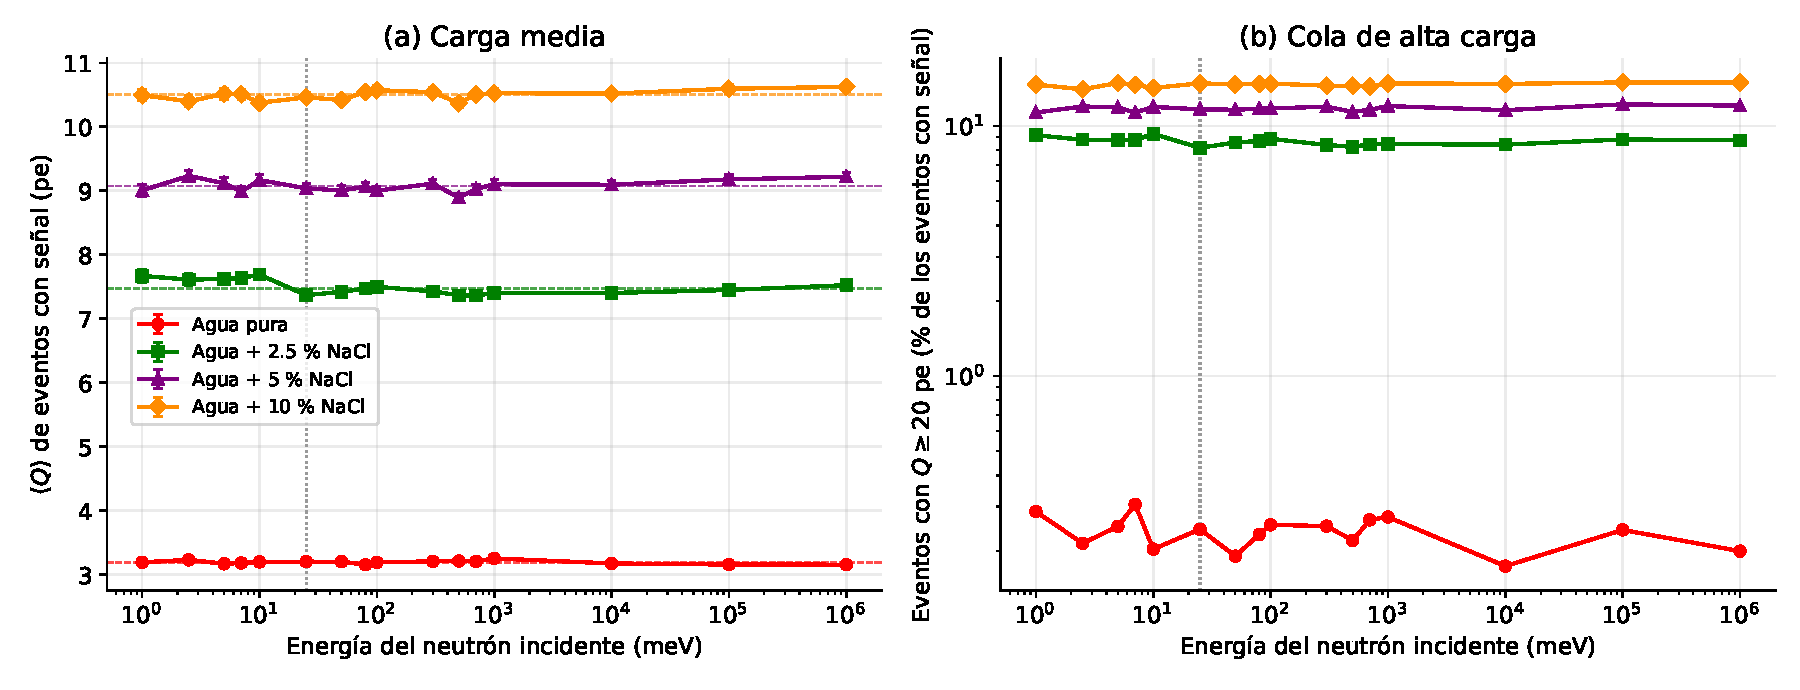
\includegraphics[width=\linewidth]{carga_vs_energia.pdf}
\caption{(a) Carga media de los eventos con señal frente a la energía del neutrón, con error estándar de la media. Las líneas discontinuas son la media ponderada de cada medio. (b) Porcentaje de los eventos con señal que tienen $Q\geq20$~pe. La línea punteada vertical marca 25~meV.}
\label{fig:carga-E}
\end{figure}

\begin{table}[H]
\centering\footnotesize\setlength{\tabcolsep}{3.5pt}
\caption{Pruebas de dependencia de la carga con la energía del neutrón. ``Media'': $\chi^2$ de las 16 cargas medias frente a una constante. ``Forma'': prueba $\chi^2$ de homogeneidad de los 16 histogramas. Última columna: diferencia entre la carga media de las energías $\leq10$~meV y la de las $\geq25$~meV.}
\label{tab:planitud}
\begin{tabular}{@{}lccccccc@{}}
\toprule
Medio & $\langle Q\rangle$ pond. (pe) & Rango (pe) & $\chi^2/\nu$ media & $p$ & $\chi^2/\nu$ forma & $p$ &
$\langle Q\rangle_{\leq10\,\mathrm{meV}}-\langle Q\rangle_{\geq25\,\mathrm{meV}}$ \\
\midrule
\input{\tablas/tabla_planitud_carga.tex} \\
\bottomrule
\end{tabular}
\end{table}

\begin{itemize}
\item \textbf{Agua pura, 5~\% y 10~\% de NaCl.} La carga media es constante dentro de la estadística ($p=0.06$, 0.08 y 0.31). La variación máxima entre energías es de 0.10, 0.34 y 0.26~pe, es decir, del 3~\% o menos. La forma completa también es compatible con ser la misma ($p=0.09$ y 0.28 en agua pura y al 5~\%). Al 10~\% la prueba de forma da $p=0.015$, pero sin tendencia en la media ($-0.06\pm0.04$~pe, $-1.4\sigma$).
\item \textbf{Agua + 2.5~\% NaCl: exceso a baja energía.} Las cinco energías $\leq10$~meV tienen una carga media de $\approx7.65$~pe; las de $\geq25$~meV, $\approx7.43$~pe. La diferencia es de $+0.22\pm0.04$~pe ($5.1\sigma$, un 3~\%), y ambas pruebas rechazan la constancia ($p=0.004$ y 0.005). El efecto \emph{no es monótono con la salinidad}: no aparece ni al 5 ni al 10~\%. Tampoco se explica por las capturas fuera del agua, porque su fracción a 1~meV es parecida en los cuatro medios (1.3--1.6~\%). Las fechas y la estructura de las carpetas de origen no muestran ninguna diferencia de producción. Queda como punto abierto; en cualquier caso es diez veces menor que la separación entre medios.
\item \textbf{Separación entre medios.} La carga media crece de forma monótona con la concentración de NaCl: $3.195\pm0.006$, $7.47\pm0.02$, $9.07\pm0.02$ y $10.50\pm0.02$~pe. Del agua pura al 2.5~\% se multiplica por 2.3; los incrementos siguientes son menores y la curva se satura.
\end{itemize}

% =====================================================================
\section{Eficiencia de detección y captura del neutrón}
\label{sec:eficiencia}

\begin{figure}[H]
\centering
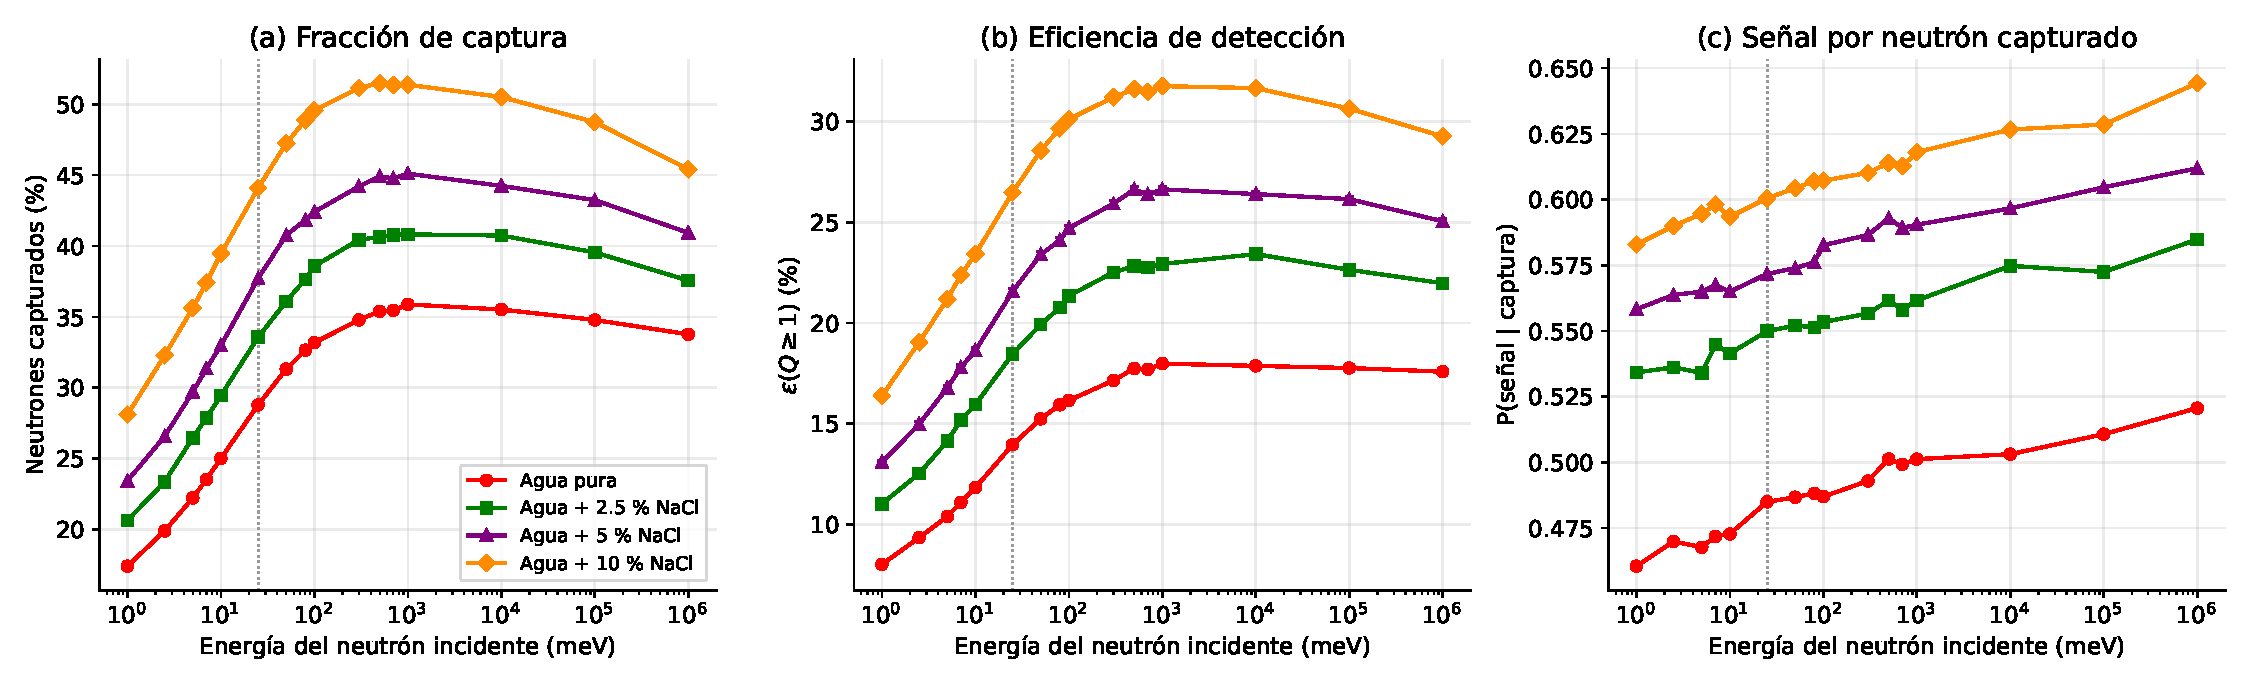
\includegraphics[width=\linewidth]{eficiencia_captura_vs_energia.pdf}
\caption{(a) Fracción de neutrones incidentes capturados, $\eta_\mathrm{Cap}$. (b) Eficiencia de detección $\varepsilon(Q\geq1)$ por neutrón incidente. (c) Probabilidad de que una captura produzca señal, $P(\text{señal}\mid\text{captura})=N(Q\geq1)/N_\text{capturas}$.}
\label{fig:eficiencia}
\end{figure}

La energía del neutrón sí cambia la eficiencia (Figura~\ref{fig:eficiencia}b):
\begin{itemize}
\item En agua pura, $\varepsilon(Q\geq1)$ sube de 8.0~\% a 1~meV a 14.0~\% a 25~meV y alcanza $\approx18$~\% entre 0.5 y 10~eV. Luego baja ligeramente, hasta 17.6~\% a 1~keV. Con 10~\% de NaCl el recorrido es de 16.4 a 31.8~\%, con máximo en 1~eV, y baja a 29.3~\% a 1~keV.
\item La mayor parte de esta dependencia viene de la \textbf{fracción de captura} (Figura~\ref{fig:eficiencia}a), que en agua pura va de 17.4 a 35.9~\%. Como se explica en el informe de flujos monocromáticos, es un efecto de albedo. Los neutrones muy lentos se termalizan cerca de la superficie del agua y la mayoría escapa por la tapa. Los más energéticos penetran antes de termalizarse y tienen más probabilidad de quedar atrapados.
\item $P(\text{señal}\mid\text{captura})$ también crece con la energía, aunque menos: de 0.46 a 0.52 en agua pura y de 0.58 a 0.64 con 10~\% de NaCl (Figura~\ref{fig:eficiencia}c). Es mayor en los medios salinos porque la cascada del cloro, más energética, produce luz con más probabilidad.
\end{itemize}

\begin{figure}[H]
\centering
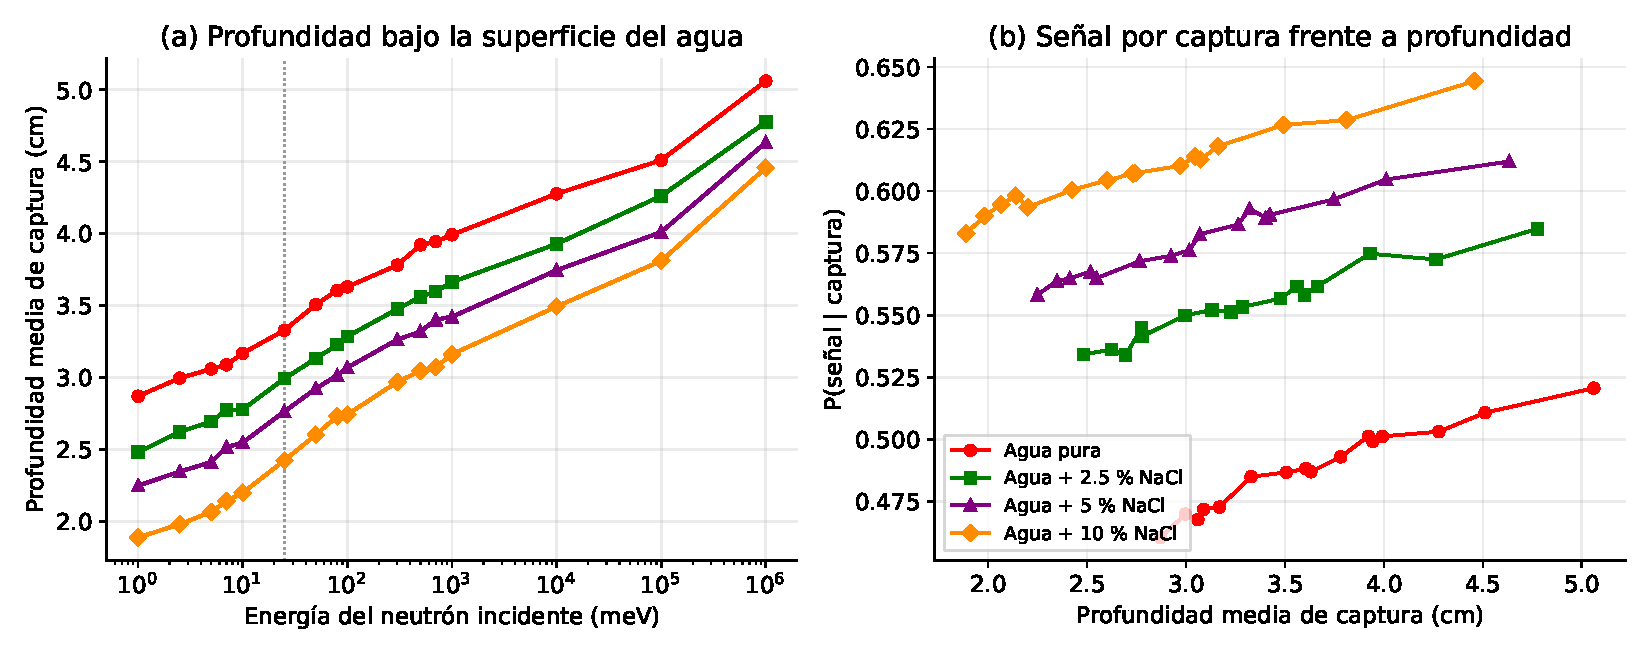
\includegraphics[width=\linewidth]{profundidad_captura.pdf}
\caption{(a) Profundidad media de captura bajo la superficie del agua frente a la energía del neutrón. (b) Probabilidad de señal por captura frente a esa profundidad media. Cada punto es una energía.}
\label{fig:profundidad}
\end{figure}

La Figura~\ref{fig:profundidad} explica el aumento de $P(\text{señal}\mid\text{captura})$. Las capturas ocurren muy cerca de la superficie del agua: a 2--5~cm de profundidad media. Esa profundidad aumenta de forma monótona con la energía, de 2.9 a 5.1~cm en agua pura. Con más sal las capturas son más superficiales, porque el cloro acorta el tiempo de vida del neutrón térmico. Cuanto más profunda es la captura, menos gammas escapan por la tapa sin interactuar, y la probabilidad de señal crece casi linealmente con la profundidad (Figura~\ref{fig:profundidad}b).

Este mecanismo cambia \emph{si} un evento da señal, pero no \emph{cuánta} carga deja cuando la da. Por eso la forma de la distribución condicionada a $Q\geq1$ (Sección~\ref{sec:carga}) es independiente de la energía.

% =====================================================================
\section{Eficiencia con umbral de carga y ganancia del NaCl}
\label{sec:umbral}

\begin{figure}[H]
\centering
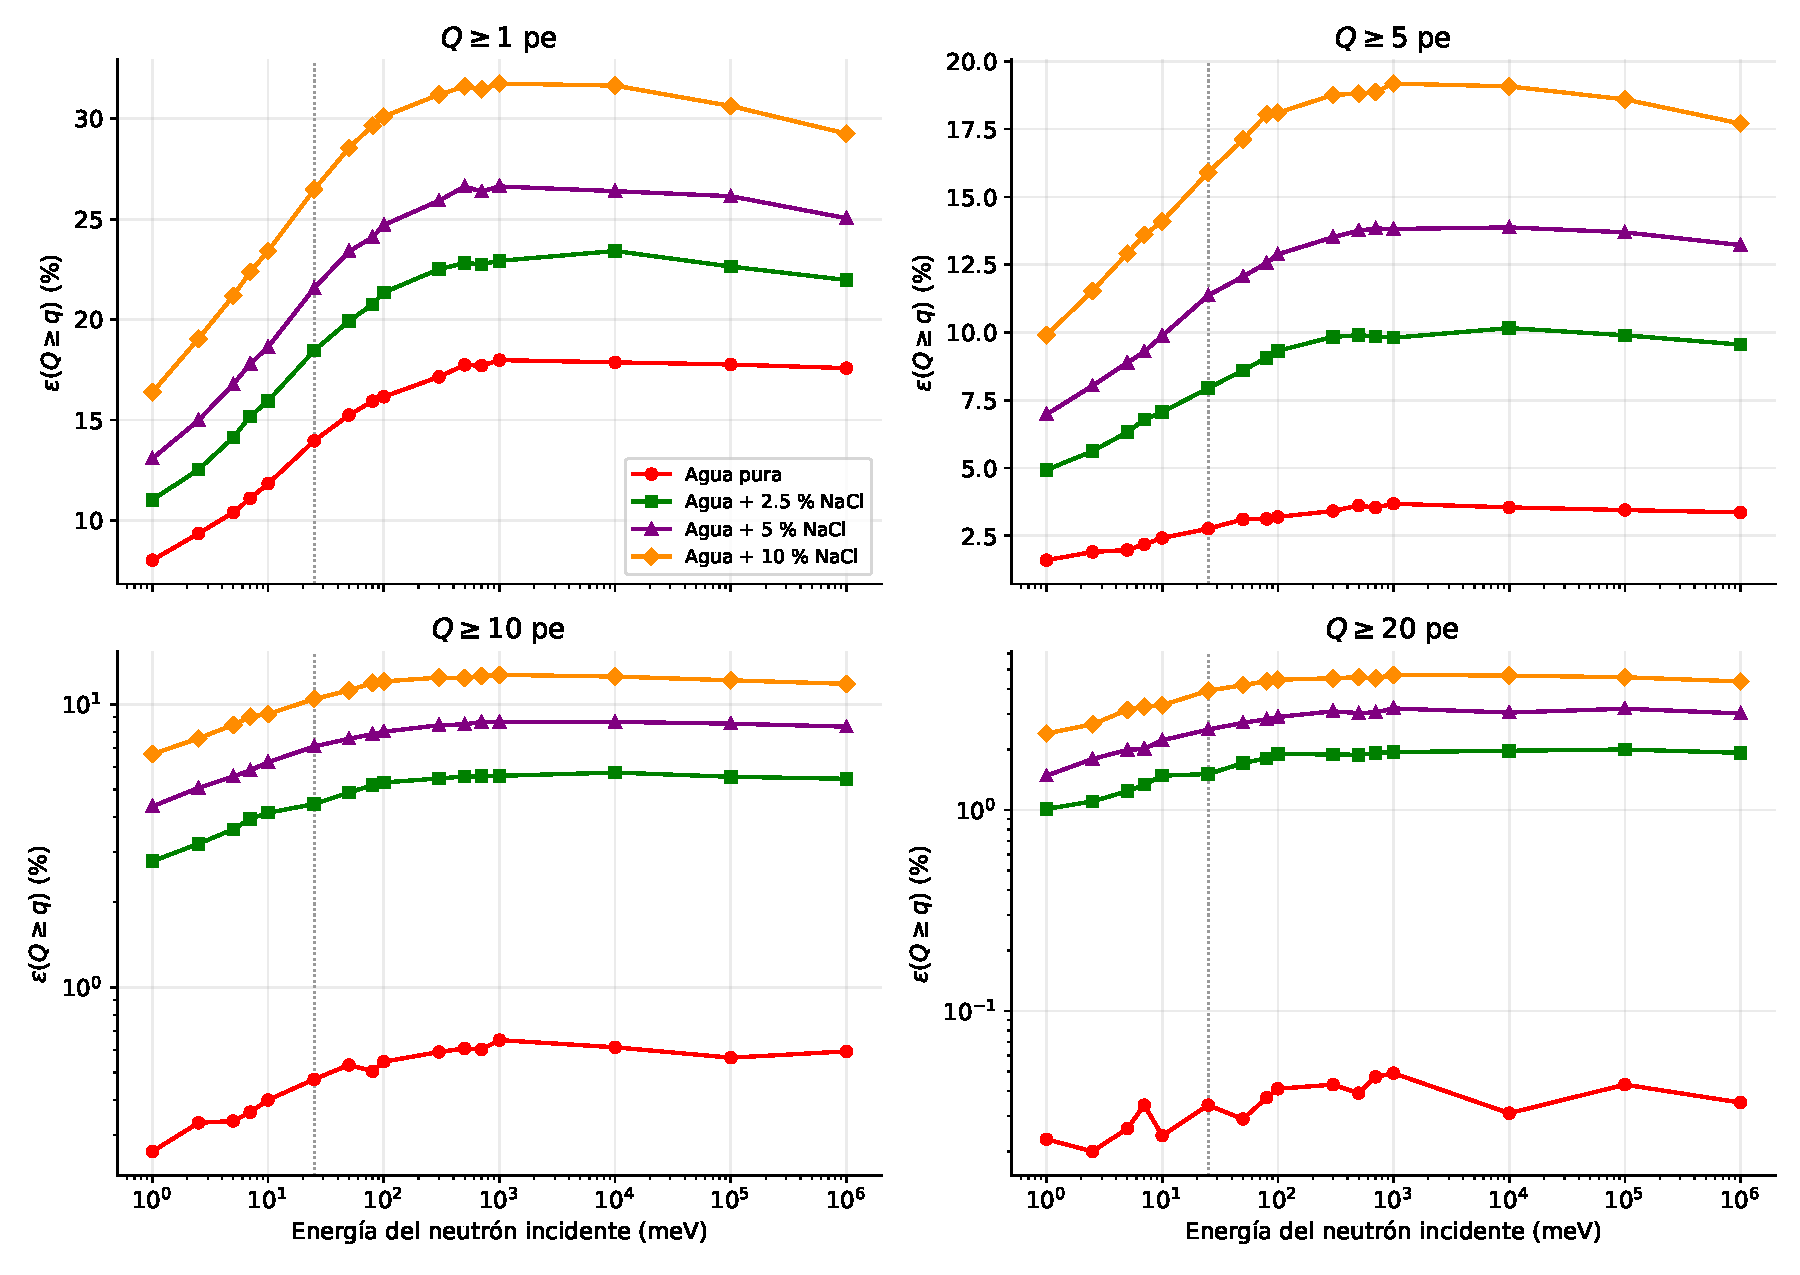
\includegraphics[width=\linewidth]{eficiencia_umbral.pdf}
\caption{Eficiencia de detección por neutrón incidente con umbrales de carga $Q\geq1$, 5, 10 y 20~pe. Los paneles de 10 y 20~pe usan escala logarítmica.}
\label{fig:umbral}
\end{figure}

\begin{table}[H]
\centering\small
\caption{Ganancia de eficiencia del agua con NaCl respecto al agua pura, $G=\varepsilon_\text{NaCl}(Q\geq q)/\varepsilon_\text{pura}(Q\geq q)$, a cuatro energías representativas. Con $Q\geq20$~pe el agua pura tiene apenas 20--50 eventos por energía, así que la última columna tiene un error relativo del 15--20~\%.}
\label{tab:ganancia}
\begin{tabular}{@{}llcccc@{}}
\toprule
Energía & Medio & $G(Q\geq1)$ & $G(Q\geq5)$ & $G(Q\geq10)$ & $G(Q\geq20)$ \\
\midrule
\input{\tablas/tabla_ganancia_eficiencia.tex} \\
\bottomrule
\end{tabular}
\end{table}

Con el umbral mínimo ($Q\geq1$), el NaCl multiplica la eficiencia por 1.25--1.37 (2.5~\%) y por 1.66--2.04 (10~\%). La ganancia es algo mayor a baja energía. Al subir el umbral la ganancia crece rápidamente, porque el agua pura apenas produce eventos de carga alta: con $Q\geq5$~pe es de $\times2.7$--$\times6.2$, y con $Q\geq20$~pe de $\times40$--$\times125$. Por tanto, un umbral de carga moderado separa con mucha eficacia las capturas en cloro de las capturas en hidrógeno y del fondo de baja carga.

% =====================================================================
\section{Tabla resumen}
\label{sec:tabla}

{\scriptsize\setlength{\tabcolsep}{3.5pt}
\begin{longtable}{@{}llrrrrrrrrr@{}}
\caption{Resumen de las 64 corridas. $N(Q\geq1)$: eventos con señal, de $10^5$ neutrones; $\varepsilon=N/10^5$; $\eta_\mathrm{Cap}$: fracción de neutrones capturados; $P(\text{s}\mid\text{c})$: eventos con señal por captura; Prof.: profundidad media de captura bajo la superficie del agua; $\langle Q\rangle$, $\sigma_Q$, Med.: media (con su error), desviación estándar y mediana de la carga de los eventos con señal; $Q\geq20$: porcentaje de los eventos con señal que superan 20~pe.}
\label{tab:resumen}\\
\toprule
$E_n$ & Medio & $N(Q\geq1)$ & $\varepsilon$ (\%) & $\eta_\mathrm{Cap}$ (\%) & $P(\text{s}\mid\text{c})$ &
Prof. (cm) & $\langle Q\rangle$ (pe) & $\sigma_Q$ & Med. & $Q\geq20$ (\%) \\
\midrule
\endfirsthead
\toprule
$E_n$ & Medio & $N(Q\geq1)$ & $\varepsilon$ (\%) & $\eta_\mathrm{Cap}$ (\%) & $P(\text{s}\mid\text{c})$ &
Prof. (cm) & $\langle Q\rangle$ (pe) & $\sigma_Q$ & Med. & $Q\geq20$ (\%) \\
\midrule
\endhead
\input{\tablas/tabla_resumen_carga.tex} \\
\bottomrule
\end{longtable}}

% =====================================================================
\section{Reproducibilidad}

Desde la carpeta \archivo{analysis/campana-1_respuesta-electromagnetica_seccion-4.2/} del repositorio:
\begin{lstlisting}
python3 procesar_carga.py ../campana-1_neutrones-monoenergeticos_seccion-4.2/resultados resultados_carga
python3 construir_notebook_carga.py
jupyter nbconvert --to notebook --execute figuras_carga_seccion_4.2.ipynb
python3 tablas_informe_carga.py resultados_carga \
  ../../docs/technical-reports/campana-1_sin-S-alpha-beta/tablas-carga
\end{lstlisting}
El procesamiento tarda unos 12~segundos. Lee los \archivo{resumen.json} de la parte neutrónica y, para la profundidad de captura, los \archivo{historias.tsv.gz}, que no están en el repositorio. Sin ellos, las columnas de profundidad quedan vacías. El notebook y las tablas funcionan solo con \archivo{resultados\_carga/}.

% =====================================================================
\section{Conclusiones}

\begin{enumerate}
\item La distribución de carga por evento en el WCD es exponencial decreciente en los 4 medios y las 16 energías de neutrón (1~meV--1~keV). Su forma y su media dependen del medio y no de la energía del neutrón: la variación entre energías es $\leq3$~\%, frente a un factor 3.3 entre agua pura y agua con 10~\% de NaCl. Es lo esperado para una señal producida por la captura radiativa tras la termalización.
\item La carga media crece de forma monótona y saturante con la salinidad: 3.2, 7.5, 9.1 y 10.5~pe. Los medios salinos muestran un hombro y una cola hasta $\sim$180~pe por la cascada de gammas del $^{35}$Cl.
\item La energía del neutrón controla \emph{cuántos} neutrones producen señal. La eficiencia $\varepsilon(Q\geq1)$ se duplica entre 1~meV y 1~eV (de 8 a 18~\% en agua pura y de 16 a 32~\% con 10~\% de NaCl). Sobre todo cambia la fracción de captura (efecto de albedo); en segundo lugar, la probabilidad de señal por captura.
\item La probabilidad de señal por captura (0.46--0.64) crece con la profundidad a la que se captura el neutrón, de solo 2--5~cm bajo la superficie, porque así escapan menos gammas por la tapa. Por eso los neutrones más energéticos, que se capturan más hondo, se detectan algo mejor.
\item El NaCl mejora la eficiencia por un factor de 1.25--2.0 con $Q\geq1$, que llega a 40--125 con $Q\geq20$~pe. Combinar NaCl con un umbral de carga es la forma más eficaz de aislar las capturas.
\item Queda abierto un exceso de carga media del $\approx3$~\% ($5\sigma$) por debajo de 10~meV en el medio con 2.5~\% de NaCl, que no aparece en los demás medios. Conviene comprobarlo repitiendo alguna de esas simulaciones con otra semilla.
\end{enumerate}
\end{document}
